\chapter{AD5941 Capacitor Selection}{}
\makeatletter\@mkboth{}{Appendix}\makeatother
\label{appen:hw_caps}

Table~\ref{tab:hw_caps} lists the capacitors around the AD5941 and the
justification for each value, as discussed in Section~\ref{sec:hw_caps}.

\begin{table}[H]
  \centering
  \caption{Capacitors around the AD5941 and the justification for each value.}
  \label{tab:hw_caps}
  \footnotesize
  \setstretch{1}
  \renewcommand{\arraystretch}{1.3}
  \setlength{\tabcolsep}{4pt}
  \begin{tabularx}{\textwidth}{@{}l l l
      >{\raggedright\arraybackslash}p{3.7cm}
      >{\raggedright\arraybackslash}X@{}}
    \toprule
    \textbf{Ref} & \textbf{Pin} & \textbf{Value} & \textbf{Role} & \textbf{Reason} \\
    \midrule
    C7, C24 & DVDD (6)   & \SI{100}{\nano\farad} & HF supply decoupling
        & Two-tier convention \cite{adi_mt101}; target impedance \cite{smith1999pds} \\
    C30 & IOVDD (26)     & \SI{100}{\nano\farad} & HF decoupling of SPI drivers
        & Two-tier convention \cite{adi_mt101}; one capacitor per pin \\
    C31 & AVDD (30)      & \SI{100}{\nano\farad} & HF supply decoupling
        & Two-tier convention \cite{adi_mt101}; local to pin 30 \\
    C33 & AVDD (41)      & \SI{100}{\nano\farad} & HF supply decoupling
        & Two-tier convention \cite{adi_mt101}; local to pin 41 \\
    C9  & AVDD (30)      & \SI{10}{\micro\farad} & Bulk decoupling; LC filter with FB1
        & Meets \SI{1}{\ohm} target above \SI{16}{\kilo\hertz} \cite{smith1999pds} \\
    C1  & \texttt{AVDD\_REG} (5) & \SI{470}{\nano\farad} & Internal LDO output capacitor
        & No datasheet value; matched to \texttt{DVDD\_REG\_1V8}
          \cite[p.~21]{ad5941_ds}, \cite{rinconmora2009ldo} \\
    C8  & \texttt{DVDD\_REG\_1V8} (14) & \SI{470}{\nano\farad} & Internal LDO output capacitor
        & Datasheet value \cite[p.~21]{ad5941_ds} \\
    C6  & \texttt{VREF\_2V5} (4) & \SI{470}{\nano\farad} & \SI{2.5}{\volt} reference decoupling
        & Datasheet value and test condition \cite[pp.~11, 20]{ad5941_ds} \\
    C10 & \texttt{VREF\_1V82} (43) & \SI{4.7}{\micro\farad} & ADC \SI{1.82}{\volt} reference reservoir
        & Datasheet recommendation \cite[p.~19]{ad5941_ds}; kickback bound \\
    C5  & \texttt{VBIAS\_CAP} (31) & \SI{470}{\nano\farad} & ADC \SI{1.11}{\volt} common-mode decoupling
        & Datasheet value and test condition \cite[pp.~11, 20]{ad5941_ds} \\
    C27 & \texttt{VBIAS0} (8) & \SI{100}{\nano\farad} & LP DAC output noise filter
        & Datasheet value \cite[p.~20]{ad5941_ds} \\
    C28 & \texttt{VZERO0} (9) & \SI{100}{\nano\farad} & LP DAC output noise filter
        & Datasheet value \cite[p.~20]{ad5941_ds} \\
    C29 & \texttt{RESET} (22) & \SI{100}{\nano\farad} & Reset hold and deglitch ($R_8 = \SI{10}{\kilo\ohm}$)
        & $\tau = \SI{1}{\milli\second} \gg \SI{1}{\micro\second}$ minimum pulse \cite[p.~14]{ad5941_ds} \\
    \bottomrule
  \end{tabularx}
\end{table}


% =====================================================================
%  Appendix -- Derivations for Chapter 3
%
%  Add to the report after \appendix with:   \input{appendix_modeling}
%  Labels referenced from system_modeling.tex:
%     app:dpv, app:feedback, app:beta, app:tia
%  Citation keys are the same as in system_modeling.tex (see its header).
% =====================================================================

\chapter{Derivations for the System Model}
\label{app:modeling}

This appendix gives the derivations behind the results used in
Chapter~\ref{chap:modeling}.

% ---------------------------------------------------------------------
\section{Capacitive Current Rejection in DPV}
\label{app:dpv}

After a potential step, the total current at the electrode is the sum of the
faradaic and capacitive components,
\begin{equation}
  I_\text{total}(t) = I_f(t) + I_c(t),
\end{equation}
with $I_c$ and $I_f$ given by Equations~\eqref{eq:ic}
and~\eqref{eq:cottrell}. Expanding the two DPV samples into these components
gives
\begin{equation}
  \Delta I = I_\text{end} - I_\text{before}
    = \left(I_{f,\text{end}} + I_{c,\text{end}}\right)
    - \left(I_{f,\text{before}} + I_{c,\text{before}}\right).
  \label{eq:app_delta_i_expanded}
\end{equation}
$I_\text{before}$ is sampled after the electrode has been held at the
baseline potential for long enough that the previous capacitive transient
has decayed, so $I_{c,\text{before}} \approx 0$. $I_\text{end}$ is sampled at
the end of a pulse that is long compared with $R_sC_{dl}$, so the transient
caused by the pulse has also decayed and $I_{c,\text{end}} \approx 0$.
Equation~\eqref{eq:app_delta_i_expanded} therefore reduces to
Equation~\eqref{eq:delta_if}, leaving only the faradaic signal.

Because $\Delta I$ is the change in faradaic current caused by a small
potential change $\Delta E$, it approximates the derivative of the
current--potential curve:
\begin{equation}
  \Delta I \approx \frac{\mathrm{d}I_f}{\mathrm{d}E}\,\Delta E.
\end{equation}
For a reversible system governed by the Nernst equation, the current--potential
curve is sigmoidal, and its derivative is a peak centred close to the
half-wave potential $E_{1/2}$, offset from it by half the pulse amplitude
\cite{bard2001, Laborda2014}.

% ---------------------------------------------------------------------
\section{Negative-Feedback Stability}
\label{app:feedback}

Both the control loop and the TIA loop have the structure of
Figure~\ref{fig:app_feedback}, where $A(s)$ is the amplifier and $\beta(s)$
is the feedback network.

\begin{figure}[htbp]
  \centering
  % KEEP: your existing control loop block diagram (old Figure 3.3).
  \caption{Control loop block diagram for the analog front-end.}
  \label{fig:app_feedback}
\end{figure}

The closed-loop transfer function is \cite{c2}
\begin{equation}
  T(s) \equiv \frac{e_o(s)}{E_\text{in}(s)} = \frac{A(s)}{1 + A(s)\beta(s)},
  \label{eq:app_closed_loop}
\end{equation}
and the loop gain is
\begin{equation}
  L(s) \equiv A(s)\beta(s).
\end{equation}
The poles of $T(s)$, which govern the transient response, are the roots of
the characteristic equation $1 + L(s) = 0$. At the crossover frequency
$\omega_c$, where $|L(j\omega_c)| = 1$, the phase margin is
\begin{equation}
  \phi_\text{PM} = \SI{180}{\degree} + \angle L(j\omega_c).
\end{equation}
If $\phi_\text{PM} \le \SI{0}{\degree}$, the closed-loop poles lie in the
right half of the $s$-plane and the system oscillates \cite{c2}.

% ---------------------------------------------------------------------
\section{Control-Loop Feedback Factor}
\label{app:beta}

In the reduced cell of Figure~\ref{fig:cell_buffer}, $R_u$ and $C_{dl}$ form
a series path from the control amplifier output $e_o(s)$ to the virtual
ground at the WE. The current through this path is
\begin{equation}
  I(s) = \frac{e_o(s)}{R_u + \dfrac{1}{sC_{dl}}},
\end{equation}
and the RE senses the voltage across the capacitive branch,
\begin{equation}
  E_\text{ref}(s) = I(s) \cdot \frac{1}{sC_{dl}}.
\end{equation}
Combining the two gives the feedback factor of Equation~\eqref{eq:beta}:
\begin{equation}
  \beta(s) \equiv \frac{E_\text{ref}(s)}{e_o(s)}
    = \frac{1}{1 + sR_uC_{dl}}.
\end{equation}
This single-pole cell model is the one used in the classical potentiostat
instrumentation literature to analyse control-loop bandwidth and
IR-compensation limits \cite{bard2001, c7, c8}.

With $A(s) = \omega_{t,\text{ctrl}}/s$, the magnitude of the loop gain in
Equation~\eqref{eq:l_ctrl} is
\begin{equation}
  |L_\text{ctrl}(j\omega)|
    = \frac{\omega_{t,\text{ctrl}}}{\omega\sqrt{1 + \omega^2\tau_\text{cell}^2}}.
\end{equation}
For $\omega\tau_\text{cell} \gg 1$ this becomes
$\omega_{t,\text{ctrl}}/(\omega^2\tau_\text{cell})$, and setting it to unity
gives Equation~\eqref{eq:wc_ctrl}. The phase of the loop gain is
$\SI{-90}{\degree} - \arctan(\omega\tau_\text{cell})$, so the phase margin is
\begin{equation}
  \phi_\text{PM,ctrl}
    = \SI{90}{\degree} - \arctan\mkern-3mu\left(\omega_{c,\text{ctrl}}\tau_\text{cell}\right)
    \approx \SI{90}{\degree} - \arctan\mkern-3mu\sqrt{\omega_{t,\text{ctrl}}\,\tau_\text{cell}},
\end{equation}
which decreases as $\tau_\text{cell}$ increases.

The RE buffer is a voltage follower, so $\beta = 1$ and
\begin{equation}
  T_\text{buf}(s) = \frac{A_\text{buf}(s)}{1 + A_\text{buf}(s)} \approx 1
  \quad \text{for } |A_\text{buf}(s)| \gg 1,
\end{equation}
so it contributes no pole over the frequency range of interest \cite{c3}.

% ---------------------------------------------------------------------
\section{TIA Transfer Function and Compensation}
\label{app:tia}

Applying Kirchhoff's current law at the inverting node of the TIA in
Figure~\ref{fig:tia}, without $C_f$, the cell current $I_\text{in}$ divides
between $C_{dl}$ and $R_f$:
\begin{equation}
  I_\text{in} = V_n\,sC_{dl} + \frac{V_n - V_\text{out}}{R_f}.
  \label{eq:app_kcl}
\end{equation}
With a finite open-loop gain, the inverting node is not exactly at zero:
\begin{equation}
  V_n = -\frac{V_\text{out}}{A(s)}.
  \label{eq:app_vn}
\end{equation}
Substituting Equation~\eqref{eq:app_vn} into Equation~\eqref{eq:app_kcl}
gives the closed-loop transimpedance
\begin{equation}
  Z_T(s) \equiv \frac{V_\text{out}}{I_\text{in}}
    = -\frac{R_f}{1 + \dfrac{1 + sR_fC_{dl}}{A(s)}}
    = -\frac{R_f}{1 + \dfrac{NG(s)}{A(s)}},
\end{equation}
which identifies the noise gain $NG(s) = 1 + sR_fC_{dl}$ of
Equation~\eqref{eq:noise_gain} and the loop gain $A(s)/NG(s)$ of
Equation~\eqref{eq:l_tia} \cite{graeme1996photodiode, adi_mt059}. Setting
$|L_\text{TIA}(j\omega)| = 1$ for $\omega R_fC_{dl} \gg 1$ gives
Equation~\eqref{eq:wc_tia} in the same way as for the control loop.

With $C_f$ in parallel with $R_f$, the feedback impedance becomes
$Z_f = R_f/(1 + sR_fC_f)$ and the noise gain becomes
\begin{equation}
  NG(s) = 1 + sC_{dl}Z_f
    = \frac{1 + sR_f\left(C_{dl} + C_f\right)}{1 + sR_fC_f}.
\end{equation}
The zero lies at $1/[2\pi R_f(C_{dl} + C_f)]$ and the new pole at
$f_p = 1/(2\pi R_fC_f)$, which is above the zero since $C_f < C_{dl} + C_f$.
Placing the pole at the geometric mean of the zero and the GBW, with
$C_f \ll C_{dl}$ so that $f_z \approx 1/(2\pi R_fC_{dl})$,
\begin{equation}
  \frac{1}{2\pi R_fC_f} = \sqrt{\frac{\text{GBW}}{2\pi R_fC_{dl}}},
\end{equation}
and solving for $C_f$ gives Equation~\eqref{eq:cf}.

\chapter{Display and SD Card Specifications}
\label{app:display_sd_specs}


\begin{table}[htbp]
  \centering
  \caption{Key specifications of the DFRobot DFR0928 display
    \cite{dfrobot_dfr0928}.}
  \label{tab:hw_display_specs}
  \begin{tabular}{@{}ll@{}}
    \toprule
    \textbf{Parameter} & \textbf{Value} \\
    \midrule
    Driver         & ST7735S \\
    Resolution     & $128 \times 160$ pixels \\
    Interface      & 4-wire SPI \\
    Supply current & \SI{33}{\milli\ampere} at \SI{3.3}{\volt} \\
    Storage        & SD card slot \\
    \bottomrule
  \end{tabular}
\end{table}

\chapter{Power Management Subsystem Specifications}
\label{app:power_specs}

\begin{table}[htbp]
  \centering
  \caption{Main specifications of the power subsystem components.}
  \label{tab:hw_power_specs}
  \small
  \begin{tabularx}{\textwidth}{@{}
      >{\raggedright\arraybackslash}X
      >{\raggedright\arraybackslash}X
      >{\raggedright\arraybackslash}X@{}}
    \toprule
    \textbf{TP4056} \cite{tp4056_ds} & \textbf{DW01A} \cite{dw01a_ds}
      & \textbf{S9V11E2F5} \cite{pololu_s9v11e2f5} \\
    \midrule
    Input supply voltage ($V_{CC}$): \SIrange{4.0}{8.0}{\volt}
      & Overcharge detection: approx.\ \SIrange{4.28}{4.30}{\volt}
      & Output voltage: fixed \SI{5}{\volt} ($+5\,\%$ / $-3\,\%$) \\
    \addlinespace
    Preset charge voltage: \SI{4.2}{\volt} with \SI{1.5}{\percent} accuracy
      & Overdischarge detection: approx.\ \SI{2.40}{\volt}
      & Input voltage range: \SIrange{2}{16}{\volt} \\
    \addlinespace
    Charge current: programmable up to \SI{1000}{\milli\ampere}
      & Overcurrent protection
      & Start-up voltage: \SI{3}{\volt}; start-up current limit:
        \SI{700}{\milli\ampere} \\
    \addlinespace
    Trickle charge threshold: \SI{2.9}{\volt}
      & Low current consumption (\SI{1.5}{\micro\ampere})
      & Typical maximum output current: up to \SI{1.7}{\ampere} \\
    \addlinespace
    Operating temperature range: \SIrange{-40}{85}{\celsius}
      &
      & Efficiency: typically \SIrange{85}{95}{\percent} \\
    \bottomrule
  \end{tabularx}
\end{table}

\chapter{Scan Flow and Timing Diagrams}
\label{app:scan_flow_timing}

\begin{figure}[H]
  \centering
  \setstretch{1}
  \begin{minipage}[b]{0.46\textwidth}
    \centering
    \begin{tikzpicture}[node distance=3mm]
      \node[swterm=26mm] (s) {Start request};
      \node[swproc=36mm, below=of s] (f) {Choose file name;\\clear point buffer};
      \node[swsub=28mm, below=of f] (r) {Select TIA range\\(Figure~\ref{fig:sw_autorange})};
      \node[swdec=22mm, below=of r] (c) {Timing\\feasible?};
      \node[swproc=36mm, below=of c] (st) {Write first base level;\\start ADC};
      \node[swsub=28mm, below=of st] (p) {Step routine\\(Figure~\ref{fig:sw_step})};
      \node[swdec=22mm, below=of p] (pt) {Point\\ready?};
      \node[swdec=22mm, below=of pt] (ov) {Overload?};
      \node[swproc=36mm, below=of ov] (rec) {Store point; update\\display and dashboard};
      \node[swdec=22mm, below=of rec] (dn) {Last\\point?};
      \node[swterm=36mm, below=of dn] (stop) {Stop ADC; $E = 0$;\\save file};
      \foreach \a/\b in {s/f, f/r, r/c, st/p, p/pt, rec/dn}
        \draw[swarr] (\a) -- (\b);
      \draw[swarr] (c) -- node[swlbl, right] {yes} (st);
      \draw[swarr] (pt) -- node[swlbl, right] {yes} (ov);
      \draw[swarr] (ov) -- node[swlbl, right] {no} (rec);
      \draw[swarr] (dn) -- node[swlbl, right] {yes} (stop);
      % loops back to the step routine
      \draw[swarr] (pt.west) -- node[swlbl, above] {no} ++(-0.55,0) |- (p.west);
      \draw[swarr] (dn.west) -- node[swlbl, above, pos=0.3] {no} ++(-0.95,0) |-
        ([yshift=2mm]p.west);
      % exits
      \draw[swarr] (ov.east) -- node[swlbl, above] {yes} ++(0.75,0) |- (stop.east);
      \node[swterm=13mm, right=8mm of c] (ab) {Refuse};
      \draw[swarr] (c) -- node[swlbl, above] {no} (ab);
    \end{tikzpicture}
    \caption{Flow of one DPV scan.}
    \label{fig:sw_scan}
  \end{minipage}\hfill
  \begin{minipage}[b]{0.53\textwidth}
    \centering
    \begin{tikzpicture}[node distance=4mm]
      \node[swterm=30mm] (e) at (0,0) {Called on every\\loop pass};
      \node[swdec=13mm] (ph) at (0,-1.45) {Phase?};
      % base branch (left column)
      \node[swdec=17mm, aspect=2] (b1) at (-2.15,-3.2)
        {$t_\text{b} - \SI{21}{\milli\second}$\\elapsed?};
      \node[swproc=32mm] (b2) at (-2.15,-5.0) {Mean of 18 samples\\$\rightarrow I_\text{before}$};
      \node[swproc=32mm] (b3) at (-2.15,-6.35) {Write pulse level;\\phase $\leftarrow$ pulse};
      % pulse branch (right column)
      \node[swdec=17mm, aspect=2] (p1) at (2.15,-3.2)
        {$t_\text{p} - \SI{21}{\milli\second}$\\elapsed?};
      \node[swproc=32mm] (p2) at (2.15,-5.0) {Mean of 18 samples\\$\rightarrow I_\text{end}$};
      \node[swproc=32mm] (p3) at (2.15,-6.35) {Compute $\Delta I$ and $E$};
      \node[swproc=32mm] (p4) at (2.15,-7.7) {Write next level;\\phase $\leftarrow$ base};
      \node[swterm=24mm] (rp) at (2.15,-9.2) {Return point};
      \node[swterm=24mm] (rn) at (-2.15,-9.2) {Return,\\no point};
      \draw[swarr] (e) -- (ph);
      \draw[swarr] (ph.west) -| node[swlbl, above, pos=0.3] {base} (b1.north);
      \draw[swarr] (ph.east) -| node[swlbl, above, pos=0.3] {pulse} (p1.north);
      \draw[swarr] (b1) -- node[swlbl, right] {yes} (b2);
      \draw[swarr] (b2) -- (b3);
      \draw[swarr] (b3) -- (rn);
      \draw[swarr] (p1) -- node[swlbl, right] {yes} (p2);
      \draw[swarr] (p2) -- (p3);
      \draw[swarr] (p3) -- (p4);
      \draw[swarr] (p4) -- (rp);
      \draw[swarr] (b1.west) -- node[swlbl, above] {no} ++(-0.3,0) |- (rn.west);
      \draw[swarr] (p1.west) -- node[swlbl, above] {no} (0,-3.2) |- (rn.east);
    \end{tikzpicture}
    \caption{Step routine. $t_\text{b} = T - t_\text{p}$ is the base
      dwell.}
    \label{fig:sw_step}
  \end{minipage}
\end{figure}

%--------------------------------------------------------------------

\chapter{RTIA Calibration Constants and Resistors}
\label{app:sw_ranges}


\begin{table}[htbp]
  \centering
  \caption{Current ranges of the high-speed TIA, the calibration constants
    held in the firmware and the resistor each range was calibrated against.}
  \label{tab:sw_ranges}
  \small
  \begin{tabular}{@{}cllllll@{}}
    \toprule
    \textbf{Code} & $R_\text{TIA}$ & \textbf{Full scale} & \textbf{Resolution}
      & $G_k$ & $O_k$ (nA) & \textbf{Cal.\ resistor} \\
    \midrule
    0 & \SI{200}{\ohm}       & $\pm\SI{4.5}{\milli\ampere}$   & \SI{187}{\nano\ampere}  & 0.9013 & $+160.04$ & \SI{994}{\ohm} \\
    1 & \SI{1}{\kilo\ohm}    & $\pm\SI{900}{\micro\ampere}$   & \SI{37.3}{\nano\ampere} & 0.9141 & $+278.66$ & \SI{994}{\ohm} \\
    2 & \SI{5}{\kilo\ohm}    & $\pm\SI{180}{\micro\ampere}$   & \SI{7.47}{\nano\ampere} & 0.9089 & $-69.54$  & \SI{4.59}{\kilo\ohm} \\
    3 & \SI{10}{\kilo\ohm}   & $\pm\SI{90}{\micro\ampere}$    & \SI{3.73}{\nano\ampere} & 0.8971 & $-81.57$  & \SI{9.93}{\kilo\ohm} \\
    4 & \SI{20}{\kilo\ohm}   & $\pm\SI{45}{\micro\ampere}$    & \SI{1.87}{\nano\ampere} & 0.9018 & $-15.8$  & \SI{19.9}{\kilo\ohm} \\
    5 & \SI{40}{\kilo\ohm}   & $\pm\SI{22.5}{\micro\ampere}$  & \SI{0.93}{\nano\ampere} & 0.9129 & $-9.159$  & \SI{38.5}{\kilo\ohm} \\
    6 & \SI{80}{\kilo\ohm}   & $\pm\SI{11.3}{\micro\ampere}$  & \SI{0.47}{\nano\ampere} & 0.9158 & $-3.014$  & \SI{81.5}{\kilo\ohm} \\
    7 & \SI{160}{\kilo\ohm}  & $\pm\SI{5.6}{\micro\ampere}$   & \SI{0.23}{\nano\ampere} & 0.9191 & $+1.005$  & \SI{146.7}{\kilo\ohm} \\
    \bottomrule
  \end{tabular}
\end{table}

\chapter{Webserver Dashboard}
\label{app:webserver_dashboard}

\begin{figure}[H]
    \centering
    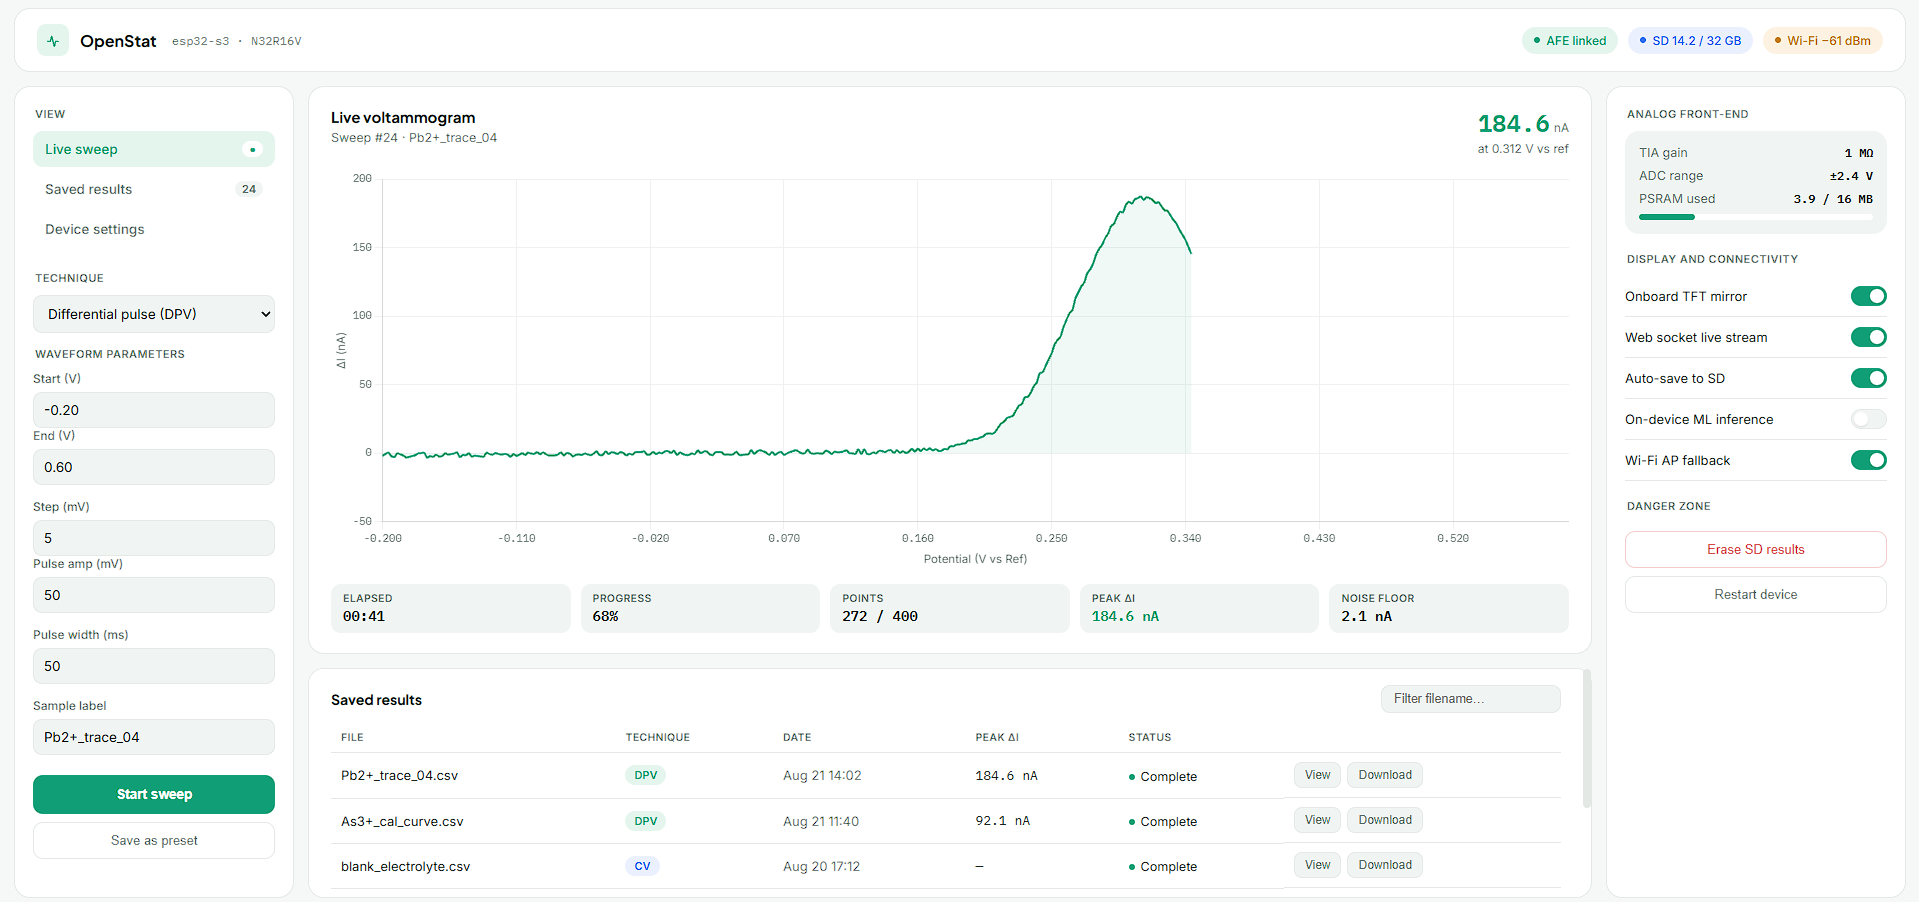
\includegraphics[width=0.7\linewidth]{figures/dashboard.png}
    \caption{The webserver dashboard for the potentiostat.}
    \label{fig:dashboard}
\end{figure}


\chapter{KiCad Schematic}
\label{app:kicad_schematic}
\begin{figure}[H]
    \centering
    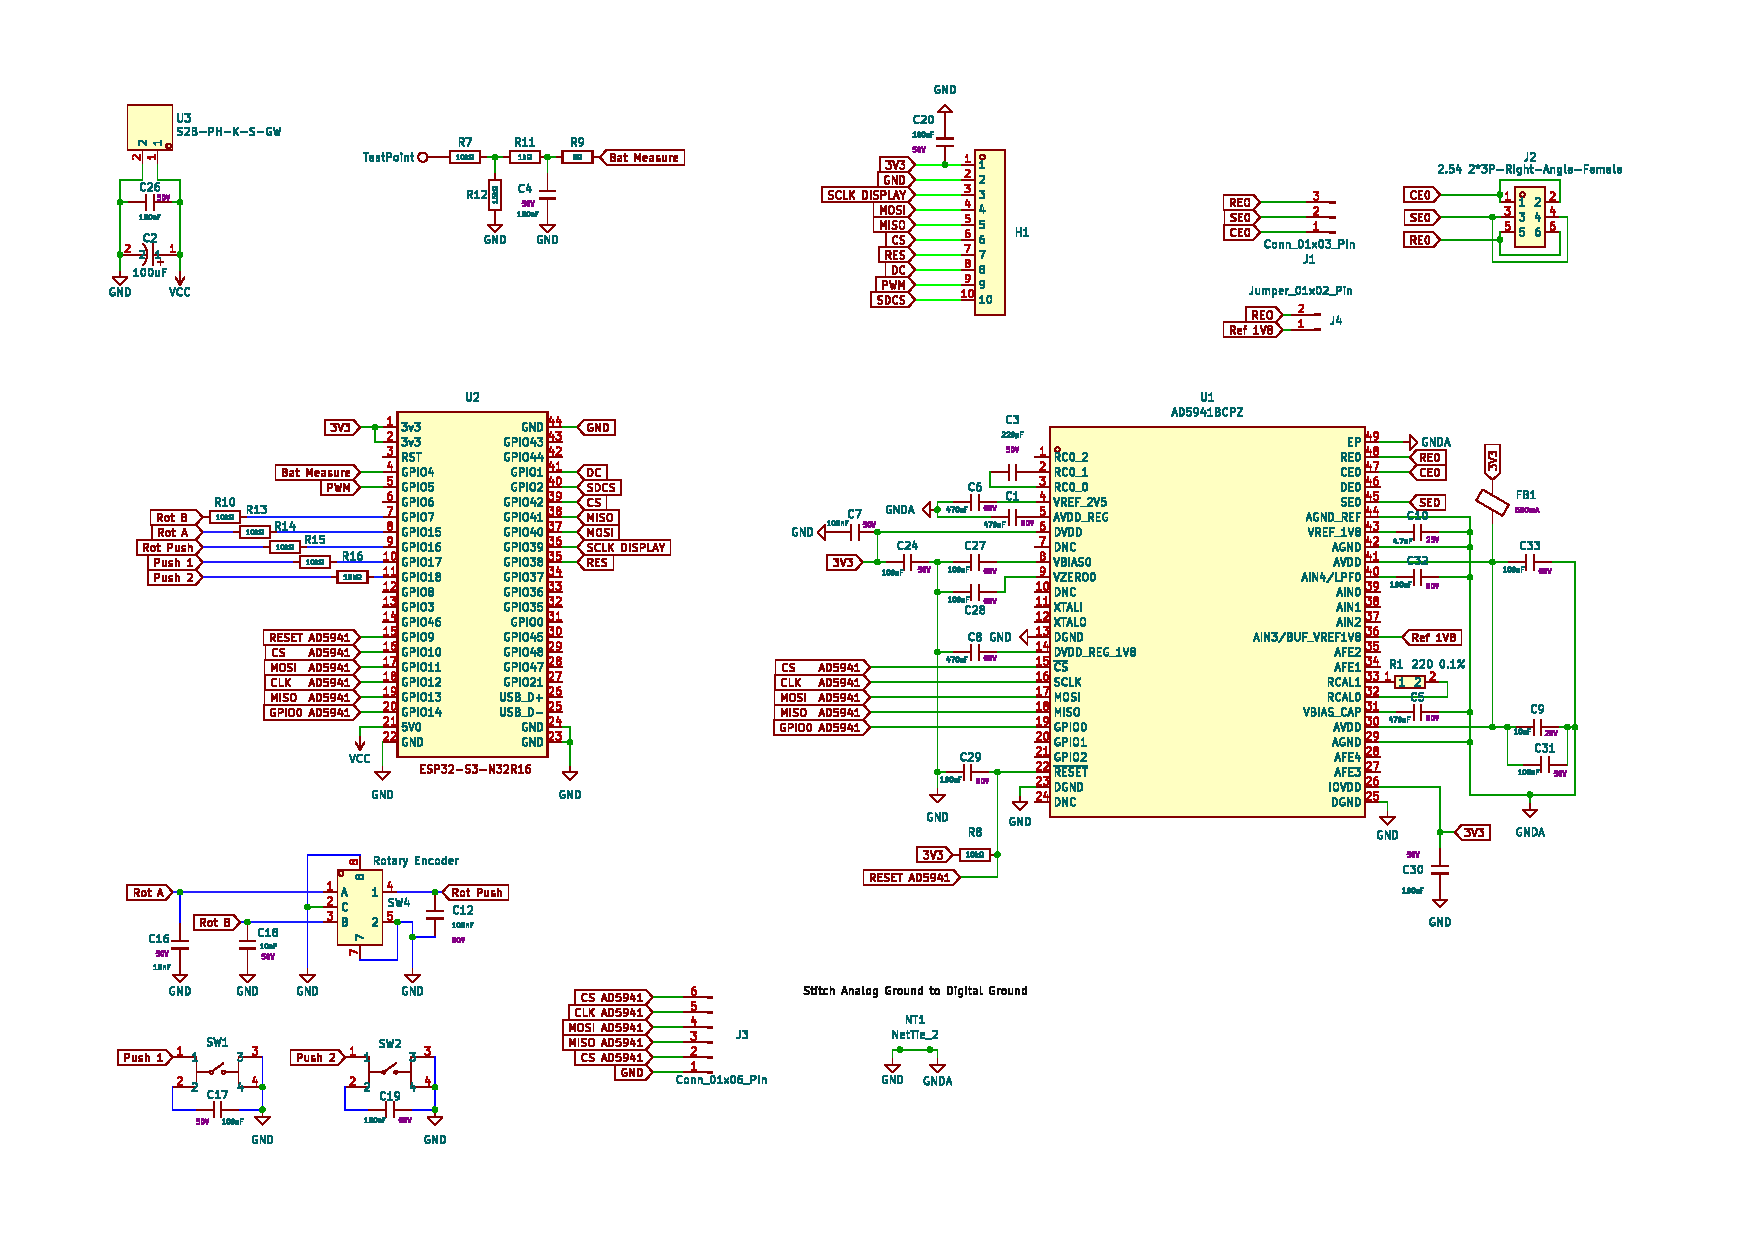
\includegraphics[angle=90, width=0.6\linewidth]{figures/KicadExport.pdf}
    \caption{The KiCad schematic for the potentiostat.}
    \label{fig:kicad_schematic}
\end{figure}

\chapter{KiCad PCB}
\label{app:kicad_pcb}
\begin{figure}[H]
    \centering
    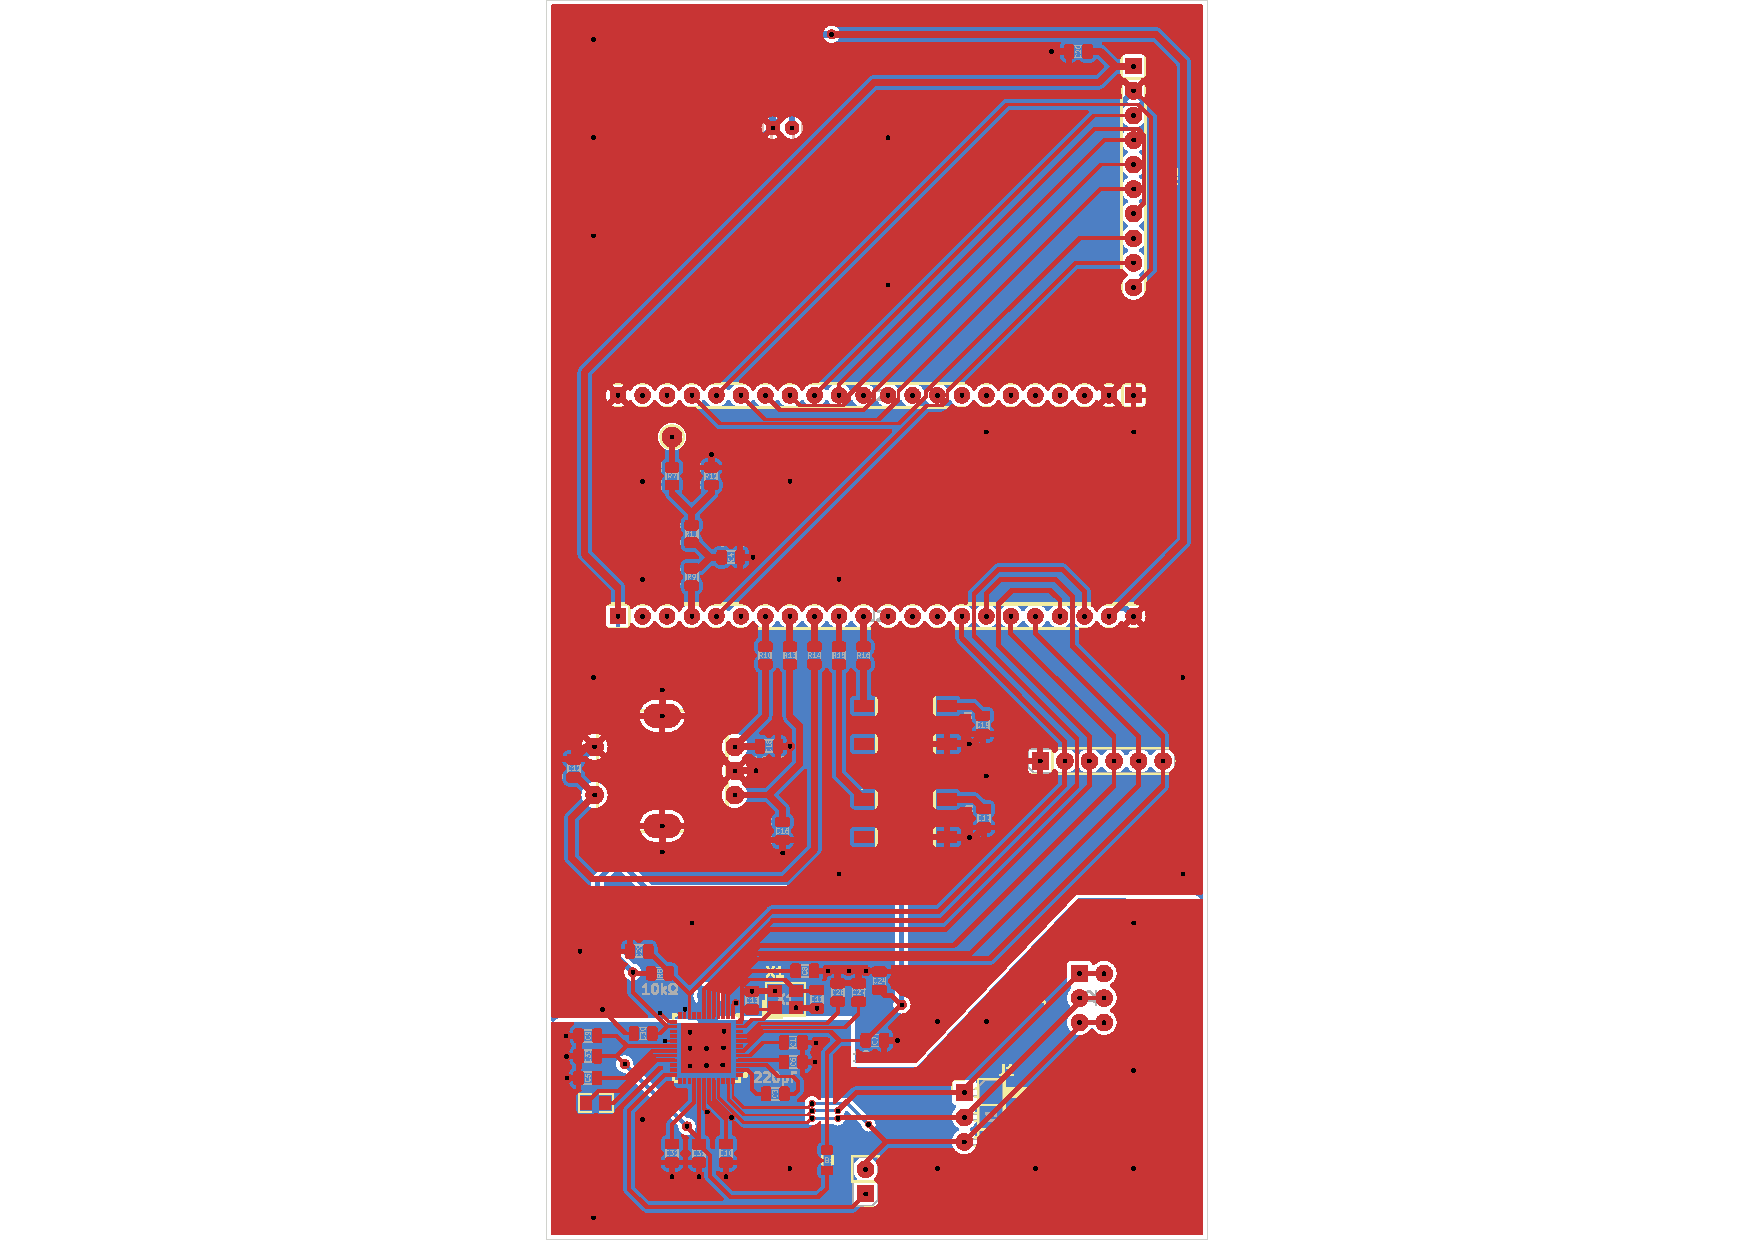
\includegraphics[angle=0, width=0.9\linewidth]{figures/pcbexport.pdf}
    \caption{The KiCad PCB for the potentiostat.}
    \label{fig:kicad_pcb}
\end{figure}


\chapter{Case Render}
\label{app:case_render}

\begin{figure}[H]
    \centering
    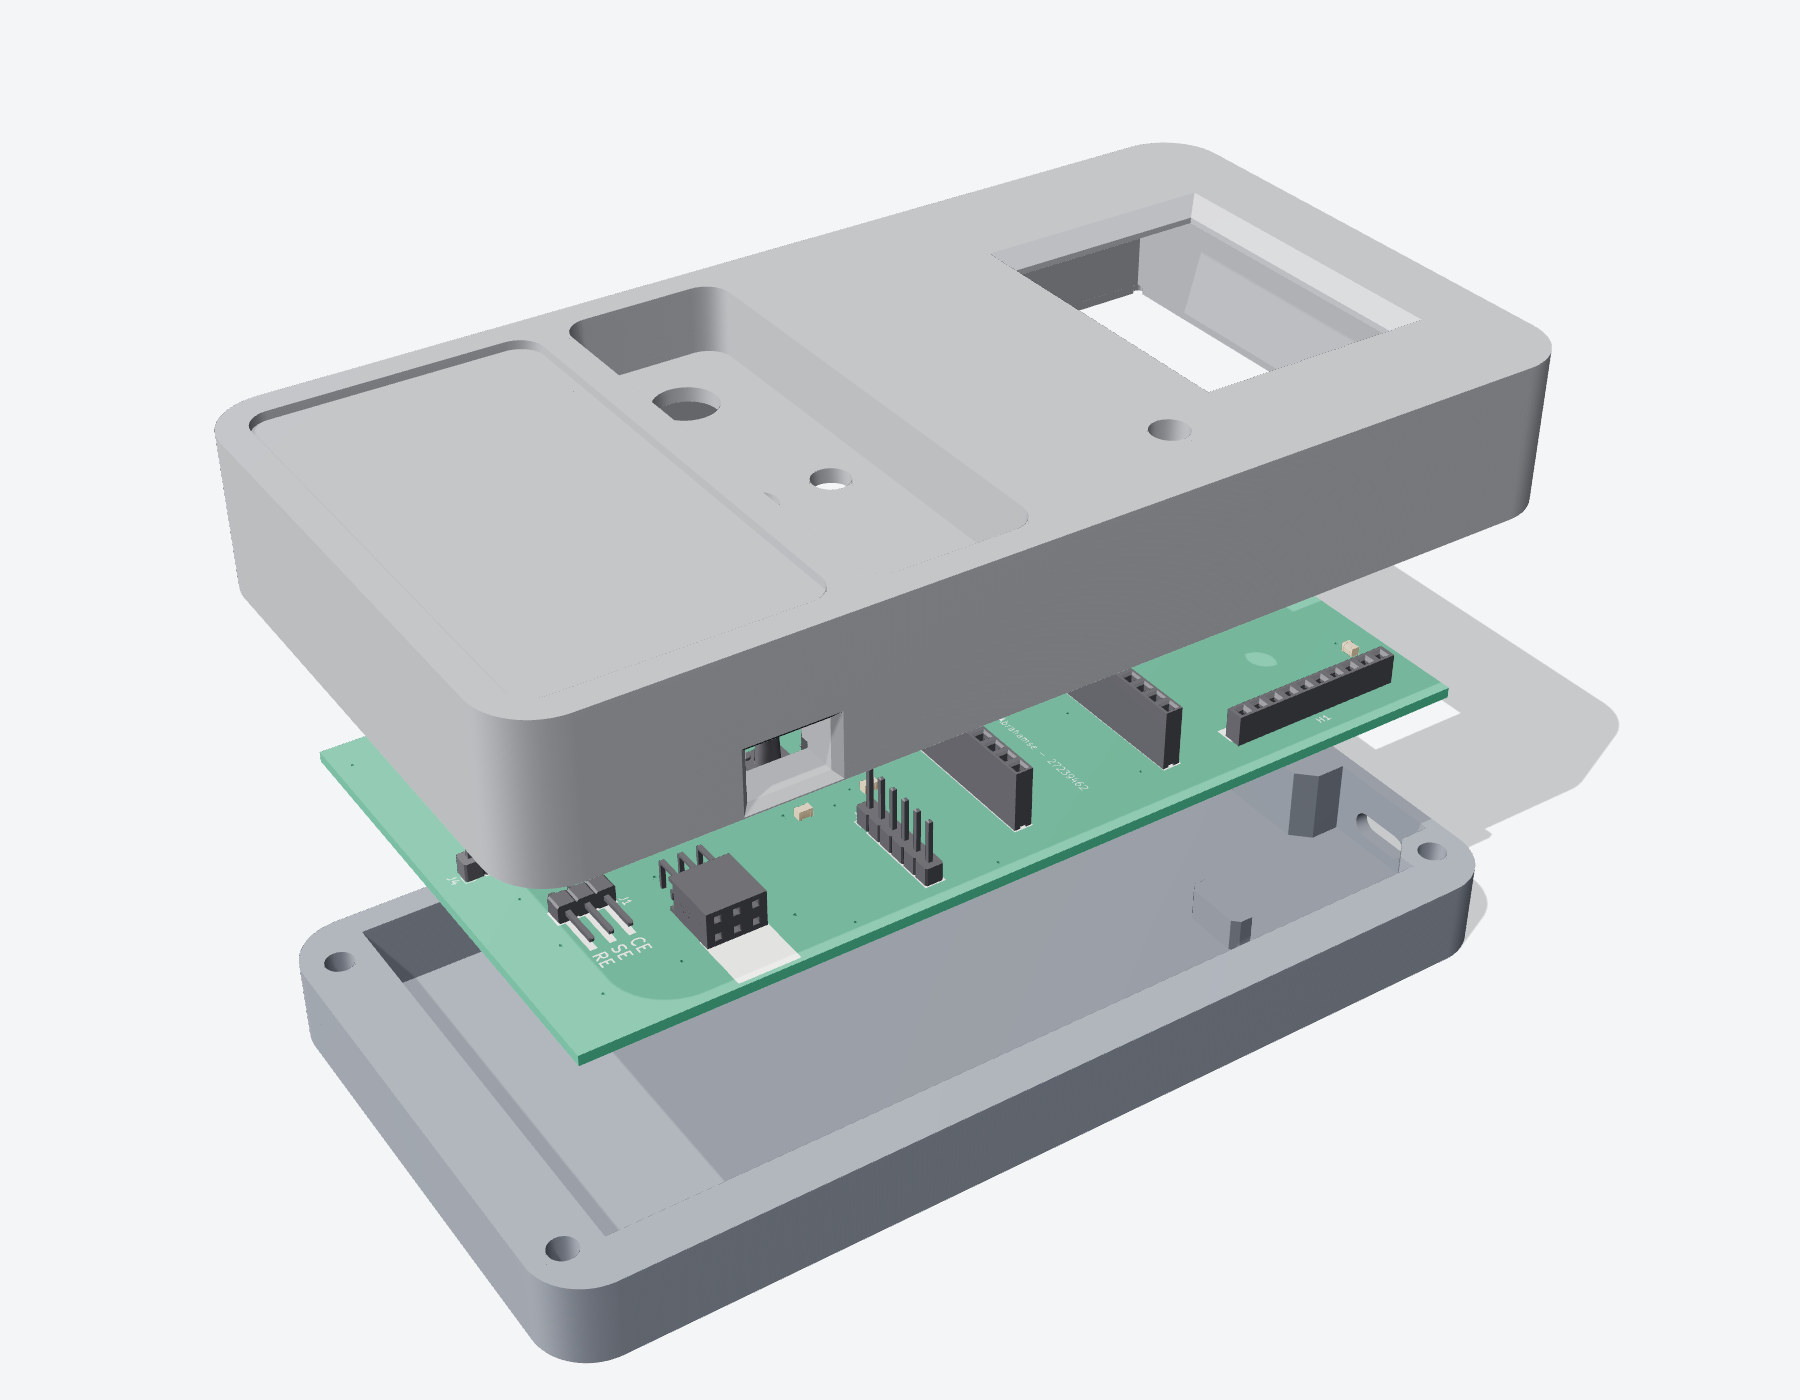
\includegraphics[width=0.7\linewidth]{figures/case model.png}
    \caption{The case render for the potentiostat.}
    \label{fig:case_render}
\end{figure}